\documentclass{beamer}
\usepackage[ngerman]{babel}
\usepackage[utf8]{inputenc}
\usepackage[]{color}
\usetheme{Malmoe}

\setbeamercovered{transparent}
\beamertemplatenavigationsymbolsempty
\setbeamertemplate{footline}[frame number]
\setbeamertemplate{sections/subsections in toc}[default]

\usecolortheme{seahorse}
\titlegraphic{
\includegraphics[width=4cm]{images/logo.png}}

\title{NEO - Ergonomisch optimiert}
\author[M. Schmidinger]{
    Markus Schmidinger
}

\begin{document}

\begin{frame}[plain]
  \titlepage
\end{frame}

\frame[plain]{
  \frametitle{Überblick}
  \tableofcontents
  [hideallsubsections]
}

\section{Geschichte}

\subsection{QWERTY}
\frame[<+->]{
  \begin{itemize}
    \item QWERTY/QWERTZ
    \item entwickelt 1868, zum Schreiben auf mechanischen Schreibmaschinen
    \item keinerlei ergonomische Optimierung
  \end{itemize}
}

\subsection{ergonomische Layouts}
\frame[<+->]{
  \begin{itemize}
    \item 1932: Dvorak 
    \item optimiert für die englische Sprache
    \item gibt auch eine deutsche Variante
  \end{itemize}
  \begin{figure}[p]
    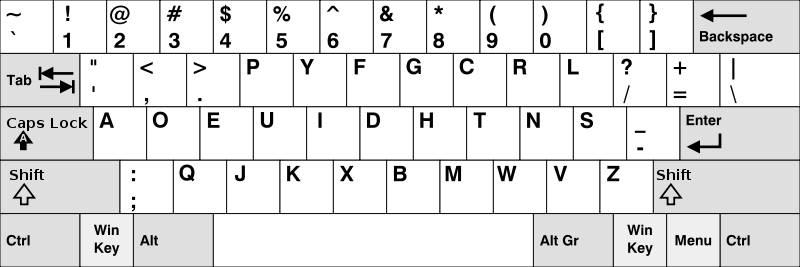
\includegraphics[width=8cm]{images/dvorak.png}
  \end{figure}
}
\frame[<+->]{
  \begin{itemize}
    \item 2003: de-ergo
    \item 2004: neo1
    \item 2010: neo2
  \end{itemize}
}

\section{Eigenschaften von NEO}
\frame[<+->]{
  \begin{itemize}
    \item Häufige Verwendung der Grundlinie
    \item Buchstabenpaare, die am häufigsten aufeinander folgen auf 2 Hände verteilt
    \item stärkere Belastung auf Zeige- und Mittelfinger
    \item Gleiche Verteilung auf linke und rechte Hand
    \item Optimierung für Deutsch, Englisch, Programmiersprachen, Shell-Befehle
    \item Sonderzeichen für Programmierung sind gut erreichbar
    \item mathematische Symbole können einfach eingegeben werden
    \item Ziffernblock, Steuerkreuz auf eigener Ebene
  \end{itemize}
}

\section{Ebenen}
\subsection{Ebene 1: Kleinbuchstaben und Zahlen}
\frame[label=Ebene1]{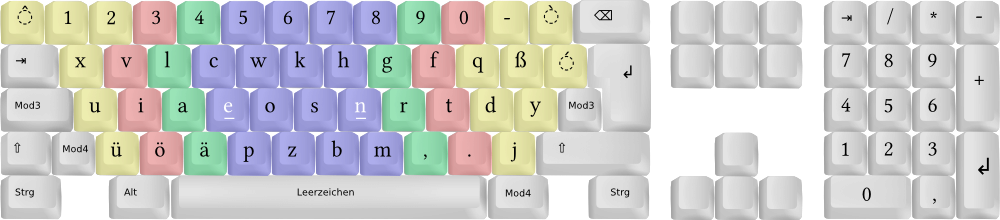
\includegraphics[width=\linewidth]{images/neo_ebene1.png}}

\subsection{Ebene 2: Großbuchstaben und Interpunktionszeichen}
\frame[label=Ebene2]{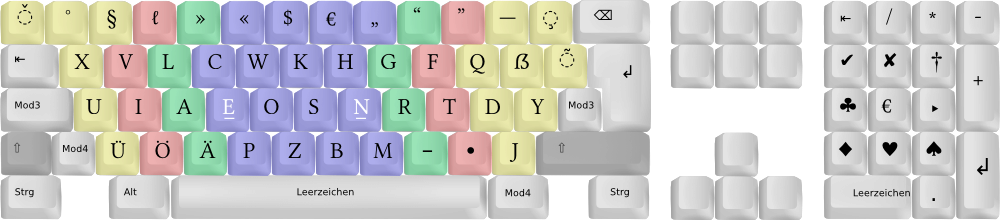
\includegraphics[width=\linewidth]{images/neo_ebene2.png}}

\subsection{Ebene 3: Sonderzeichen und weitere Interpunktionszeichen}
\frame[label=Ebene3]{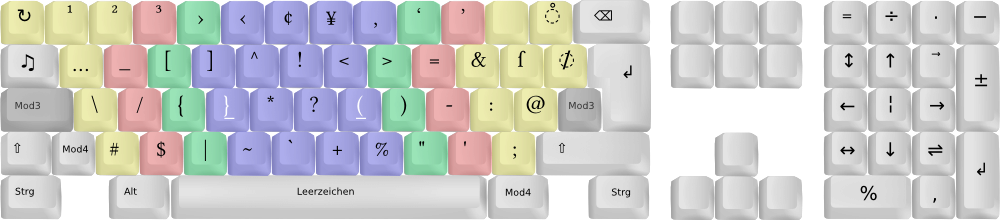
\includegraphics[width=\linewidth]{images/neo_ebene3.png}}

\subsection{Ebene 4: Navigationstasten und Zahlen}
\frame[label=Ebene4]{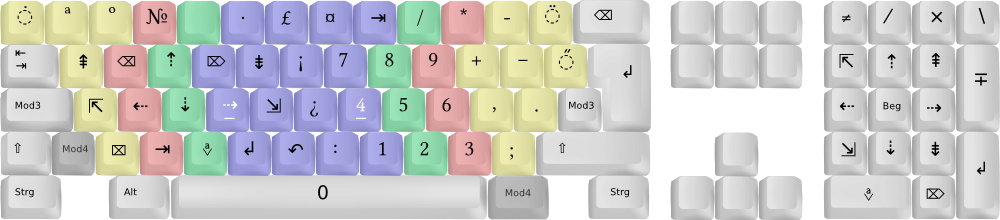
\includegraphics[width=\linewidth]{images/neo_ebene4.png}}

\subsection{Ebene 5: Griechische Kleinbuchstaben}
\frame[label=Ebene5]{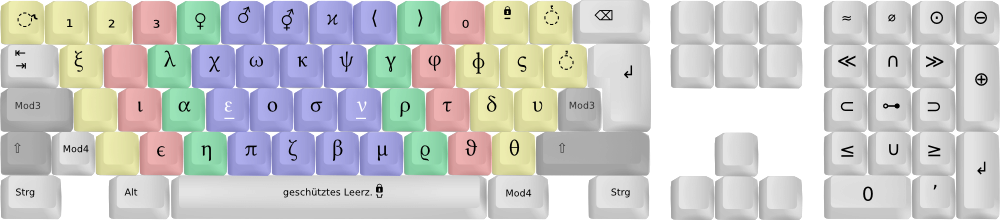
\includegraphics[width=\linewidth]{images/neo_ebene5.png}}

\subsection{Ebene 6: Wissenschaftliche Zeichen und Griechische}
\frame[label=Ebene6]{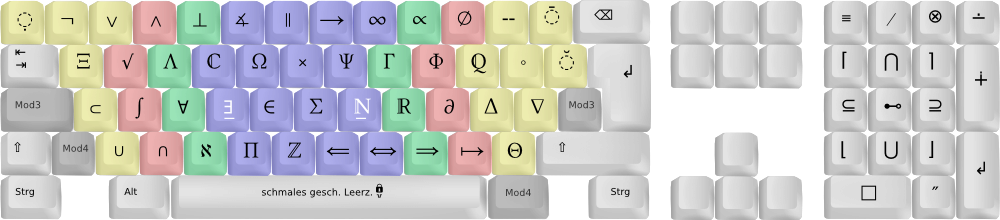
\includegraphics[width=\linewidth]{images/neo_ebene6.png}}

\section{Vergleich Homerow}

\subsection{QWERTZ - Linux - Deutsch}
\frame{ 
  \input{tools/linux_ger.txt_qwertz}
}
\subsection{NEO - Linux - Deutsch}
\frame{
  \input{tools/linux_ger.txt_neo}
}

\subsection{QWERTZ - Linux - Englisch}
\frame{ 
  \input{tools/linux_eng.txt_qwertz} 
} 

\subsection{NEO - Linux - Englisch}
\frame{
  \input{tools/linux_eng.txt_neo}
}

\subsection{QWERTZ - Python - Deutsch}
\frame{
  \input{tools/python_ger.txt_qwertz}
}

\subsection{NEO - Python - Deutsch}
\frame{
  \input{tools/python_ger.txt_neo}
}

\section{Vergleich Handwechsel}
\subsection{QWERTZ - Linux - Deutsch}
\frame{
  \input{tools/linux_ger.txt_handchange_qwertz}
}
\subsection{NEO- Linux - Deutsch}
\frame{
  \input{tools/linux_ger.txt_handchange_neo}
}

\section{Kompatibilität}
\frame{
  \begin{itemize}
    \item Linux
      \begin{itemize}
        \item Terminal: setxkbmap de neo
        \item Systemweite Installation (Xkbmap)
        \item Auf der Textkonsole
      \end{itemize}
    \item Windows 
      \begin{itemize}
        \item NeoVars-Treiber (ohne Adminrechte)
        \item kbdneo-Treiber
      \end{itemize}
    \item MacOS
    \item FreeBSD, OpenBSD, NetBSD
    \item Commodore 64 (Version 1.0)
    \item …
  \end{itemize}
}

\section{Zukunft}
\frame[<+->]{
  \begin{itemize}
    \item neo3(?), adnw, bone, ...
    \item ergonomische Tastaturen
  \end{itemize}
}

\frame{
  \begin{figure}[p]
    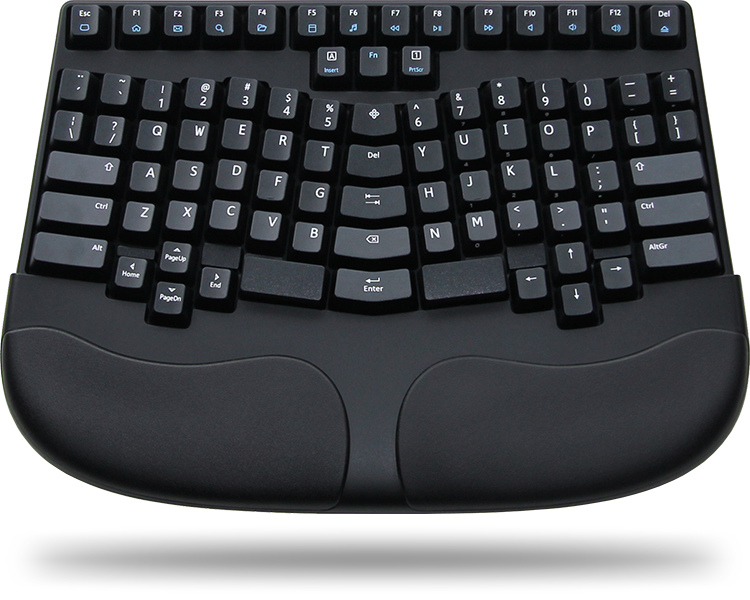
\includegraphics[width=6cm]{images/truly}
  \end{figure}
}

\frame{
  \begin{figure}[p]
    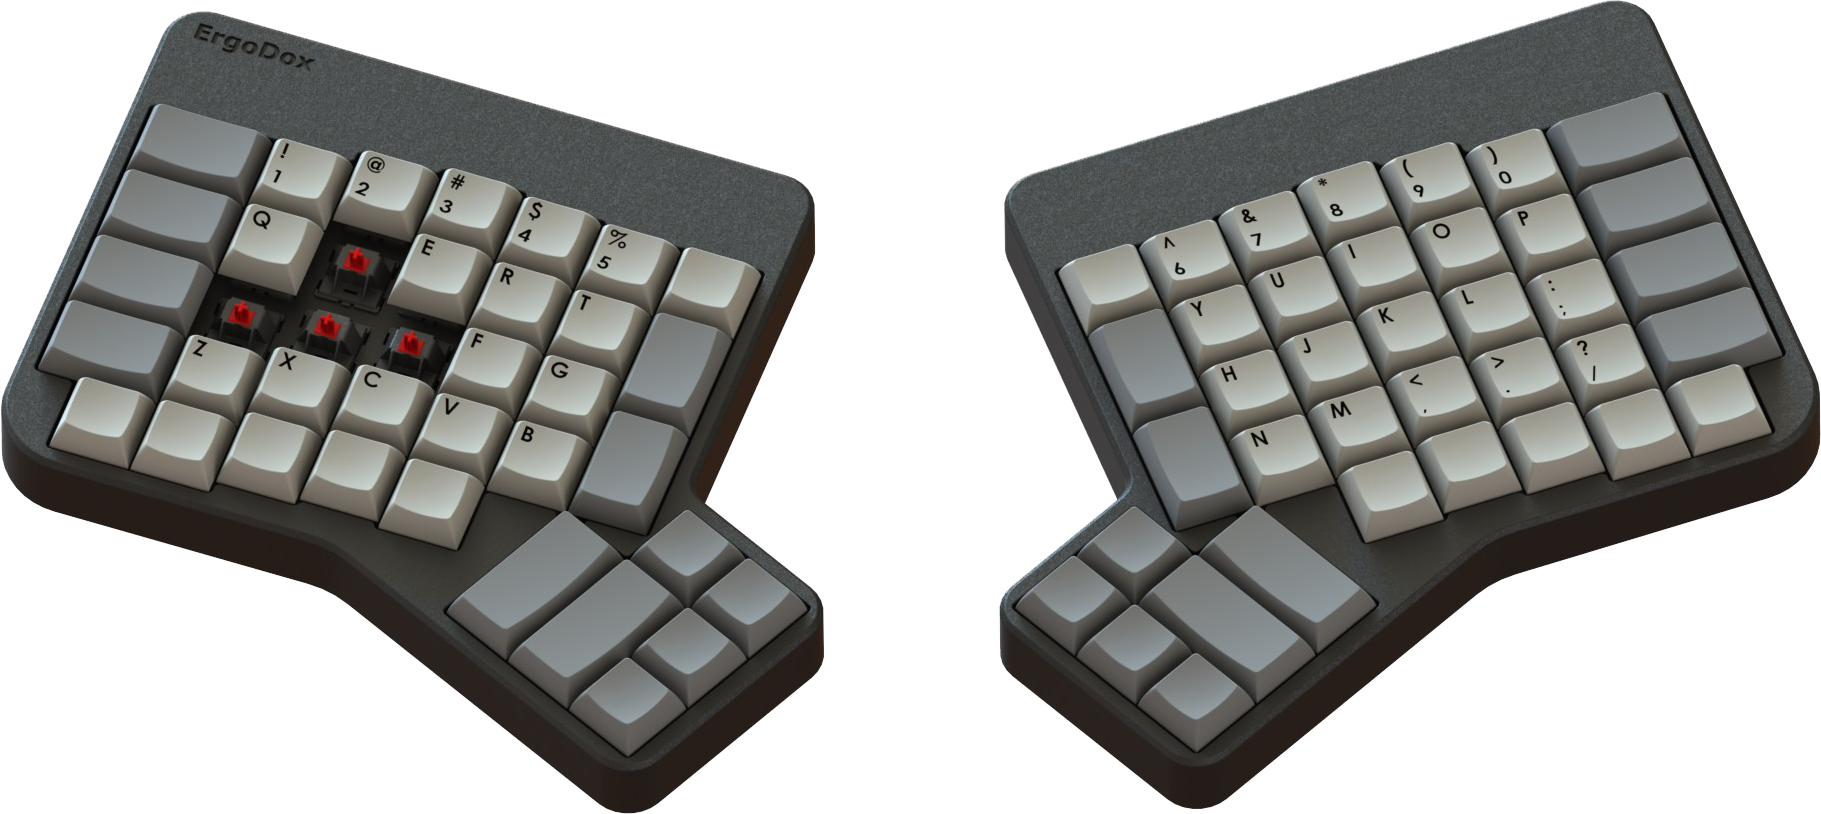
\includegraphics[width=8cm]{images/ergodox}
  \end{figure}
}

\end{document}
